\section{Contexto del sistema}
\label{sec:contexto}

\subsection{Límite del sistema y contexto propuesto}
El límite del Sistema de Gestión para Restaurante con IA (SGR-IA) se ubica en la interfaz entre la operación de sala, cocina, caja e inventario de El Balcón Restaurant y las personas que interactúan con ella. La figura~\ref{fig:contexto} presenta las entidades externas y los flujos de información identificados a partir del dominio del negocio y de cuatro entrevistas de campo aplicadas con la guía corregida de 45 preguntas. La cláusula 6.3.3.2 de ISO/IEC/IEEE 29148:2018 dispone identificar a las partes interesadas a lo largo del ciclo de vida y definir una estrategia para elicitar sus necesidades y transformarlas en requisitos \cite{iso29148}; en coherencia con ese criterio, el diagrama distingue las entidades que interactúan con el sistema de los sistemas externos que quedan fuera de alcance, como la facturación electrónica.

\begin{figure}[htbp]
\centering
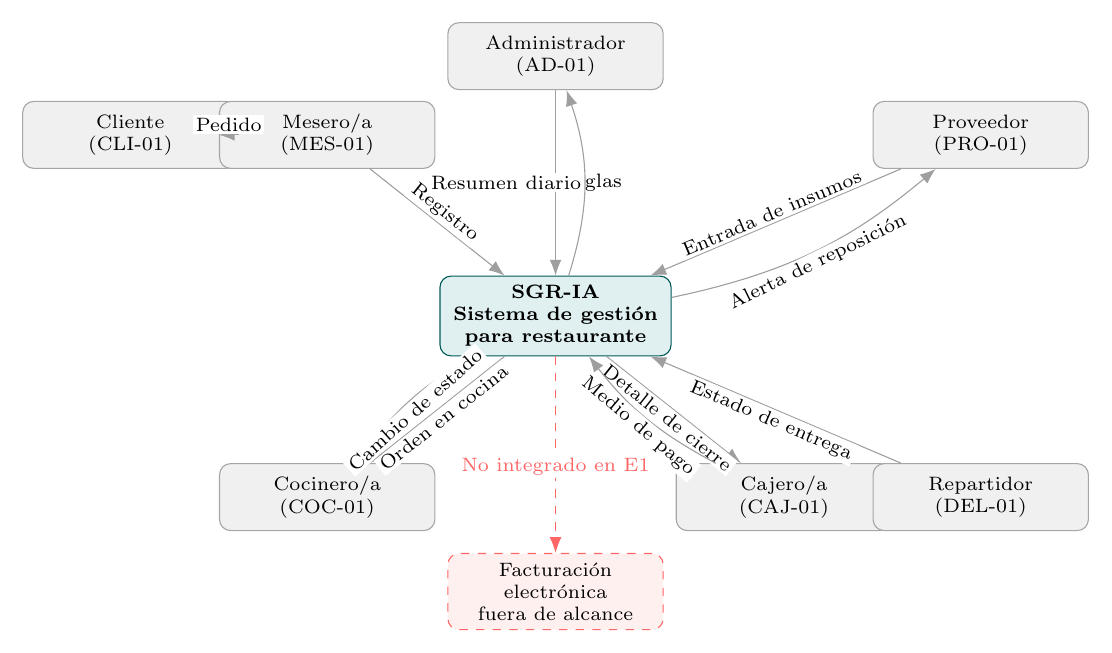
\includegraphics[width=0.90\linewidth]{figuras/contexto.png}
\caption{Contexto del SGR-IA y entidades externas.}
\label{fig:contexto}
\end{figure}

\subsection{Participantes de campo y trato de la información}
Las transcripciones corregidas \texttt{ENTR-01} a \texttt{ENTR-04} son evidencia de campo obtenida por el equipo en El Balcón Restaurant. Usan únicamente códigos de participante y no contienen nombres, cédulas, teléfonos ni correos. Por decisión de custodia, las transcripciones y grabaciones permanecen en carpeta privada `@uteq.edu.ec`; en este documento solo se usan paráfrasis anónimas, sin citas textuales, porque `ENTR-02` no autorizó citar frases literalmente ni depositar sus datos en un repositorio abierto. Los originales firmados de los cuatro formularios de consentimiento se recibieron el 21/11 y se custodian en la carpeta privada `@uteq.edu.ec`; sus nombres, fechas y huellas constan en el manifiesto. La fecha manuscrita de cada formulario no puede leerse con fiabilidad en la copia digital, por lo que no se afirma que el consentimiento haya sido previo a las sesiones. Las fechas informadas son 18/11 (ENTR-01), 19/11 (ENTR-02), 20/11 (ENTR-04) y 21/11 (ENTR-03); las duraciones constan en el manifiesto. Adem\'as de los videos, se recibieron los audios de las cuatro sesiones en \texttt{audio.p.zip}; se conservan en la carpeta privada con los mismos c\'odigos \texttt{ENTR-01} a \texttt{ENTR-04}. Sus duraciones y huellas SHA-256 figuran en el manifiesto como EV-18 a EV-21. El informe no reproduce fragmentos de audio ni datos personales de los participantes.

\begin{table}[htbp]
\centering
\footnotesize
\begin{tabularx}{\linewidth}{|p{1.7cm}|X|p{2.0cm}|p{2.5cm}|}
\hline
\thdr{Código} & \thdr{Rol declarado} & \thdr{Antigüedad} & \thdr{Volumen informado (normal / alto)}\\
\hline
ENTR-01 & Administradora & 1 año 1 mes & 25--30 / 50 personas\\
\hline
ENTR-02 & Cocinera & 2 años & 25 / 35 platos\\
\hline
ENTR-03 & Auxiliar de cocina & 3 años & 45 / 85 pedidos\\
\hline
ENTR-04 & Cajera & 3 años & 60 / 120 pedidos\\
\hline
\end{tabularx}
\caption{Participantes de campo y volúmenes informados por rol.}
\label{tab:participantes}
\end{table}

Los roles de la tabla~\ref{tab:participantes} fueron informados por el equipo
el 21/11; las transcripciones conservan su redacción original y no se han
modificado para ajustarlos.

Las cifras de la tabla~\ref{tab:participantes} no son homogéneas: cada persona mide una unidad distinta (personas, platos o pedidos) en días diferentes. Por ello no se promedian ni se presentan como un dato único de la organización; quedan sujetas a confirmación con el responsable. Las fechas y duraciones reales, tomadas de las grabaciones y de lo informado por el equipo, se registran en el manifiesto; dos de los videos llevan en su título original el nombre del líder, quien realizó y grabó las entrevistas.

\subsection{Ocho perspectivas de análisis del contexto}
La tabla~\ref{tab:perspectivas} actualiza las ocho perspectivas con los hallazgos de campo disponibles. Cuando la información solo proviene de la propuesta inicial se conserva la etiqueta \emph{propuesta}; cuando proviene de las entrevistas se indica el código del participante. Ninguna celda afirma una meta cuantitativa acordada con el responsable, porque esa validación aún no se ha realizado.

\begin{table}[htbp]
\centering
\footnotesize
\begin{tabularx}{\linewidth}{|p{2.5cm}|X|p{2.0cm}|}
\hline
\thdr{Perspectiva} & \thdr{Hallazgo de campo o propuesta} & \thdr{Estado}\\
\hline
Objetivos de negocio & Reducir espera y errores; dolencias: cierre de caja de unas 1--2 h (ENTR-04), conteo de insumos (ENTR-03) y avisos de días sin servicio (ENTR-01). & Parcial\\
\hline
Usuarios y roles & Administradora (ENTR-01), cocinera (ENTR-02), auxiliar de cocina (ENTR-03) y cajera (ENTR-04). Deciden la jefa o el encargado; equipo de 3 a 7 personas. & Campo\\
\hline
Tareas y flujos & Comanda en papel, cocina y caja (ENTR-01/04); domicilio por WhatsApp y moto (ENTR-01/03); cambios comunicados de palabra y no anotados (ENTR-03/04). & Campo\\
\hline
Información y datos & Cuaderno, libreta, pizarra y planilla final; errores por letra poco clara y pedidos modificados sin registro (ENTR-04); stock no se actualiza de inmediato (ENTR-03). & Campo\\
\hline
Funciones del sistema & Registro de pedidos, reservas, inventario, caja y reportes; facturación electrónica permanece fuera del límite (sección~\ref{sec:alcance}). & Propuesta\\
\hline
Comportamiento y estados & Pedido tomado, en cocina, listo y cobrado; domicilio tomado, preparado, en reparto y entregado (ENTR-03/04). Hoy no hay estados informáticos. & Parcial\\
\hline
Calidad y atributos & Errores «pocas veces al mes» (ENTR-01/02/04); la espera y el cobro concentran las molestias; se requiere cuidado con datos de personal y clientes (ENTR-01/03/04). & Campo\\
\hline
Restricciones e interfaces & WhatsApp, efectivo, transferencia y tarjeta, reparto en moto, conectividad y SRI; seis proveedores (ENTR-03); recetas no escritas (ENTR-03/04). & Parcial\\
\hline
\end{tabularx}
\caption{Ocho perspectivas del contexto actualizadas con entrevistas de campo.}
\label{tab:perspectivas}
\end{table}

La tabla~\ref{tab:perspectivas} será revisada con el responsable de la organización para cerrar metas medibles, estados autorizados y prioridades. Las celdas marcadas como \emph{parcial} o \emph{propuesta} no deben interpretarse como acuerdos validados.
